\documentclass{standalone}

\begin{document}

\subsection{Background Theory\label{sec:method:background}}

To approach the problem, the first step was to begin with establishing the parameters that will be used to characterize both the parameters of the input and the format to describe the output.
This was done by establishing two coordinate systems: the \emph{observer's sky} and the \emph{source sky}, and are charted via spherical coordinates.

Physically, the observer's sky is defined as the past lightcone at the location of the observer, meaning that the light that is observed at this point describes the set of null-geodesics that have been emitted from the source sky that cross with the observer.
Therefore, describing the lensing due to the curvature of spacetime amounts to solving the null-geodesic equation using the observer as the initial condition:
\begin{eqnarray}
  \dv[2]{x^\mu}{\lambda} + \Gamma^\mu_{\rho\sigma}\dv{x^\rho}{\lambda}\dv{x^\sigma}{\lambda} = 0,\label{eq:geodeq}\\
  g_{\mu\nu}\dv{x^\mu}{\lambda}\dv{x^\nu}{\lambda} = 0.\label{eq:nullcondition}
\end{eqnarray}
Where $x^\mu$ characterizes the path of the light through spacetime, $\lambda$ is an arbitrary choice of an affine parameter, $g_{\mu\nu}$ is the spacetime metric, and $\Gamma^\mu_{\rho\sigma}$ are the Christoffel symbols.

Now, to characterize the problem, our goal is to map angles, $(\theta,\phi)$, on the observer's sky to the output angles $(\psi,\gamma)$ on the source sky.
A mathematical simplification for spherically symmetric lenses is to define a new angle, $\Theta$, that is defined as the angle between the point $(\theta,\phi)$ and the optical axis that is drawn from the center of the lens to the observer.\cite{gen_lens}
This reduces the problem to finding how $\Theta$ maps to $\Phi$, the angle between the source $(\psi,\gamma)$ and the same optical axis used to define $\Theta$.
These parameters are illustrated in Fig.(\ref{fig:mappingdiagram}).

\begin{figure}[hb]
  \caption{\label{fig:mappingdiagram}
    Illustration of the process we intend to describe (inspired by a figure used in \cite{gen_lens}).
    The center of the two concentric circles defines the center of the lens.
    $r_O$ and $r_S$ are the radial distance from the lens' center two the observer and the collection of sources respectively.
    The curve between the two radii represents the path that was traveled by a light ray that was emitted at the point at the angular position $\Phi$ relative to the optical axis and is absorbed by the observer at the angle $\Theta$.
  }
  \vspace{3mm}
  \begin{tikzpicture}[scale=1.5,>=stealth]
    \small
    \def\sourceangle{110}
    \def\thetaangle{30}
    \def\alphaangle{0}
    \def\Ro{4mm}
    \def\Rs{16mm}
    \draw[thick] (0,0) circle (\Ro);
    \draw[thick] (0,0) circle (\Rs);
    \coordinate (Ro) at (\Ro,0);
    \coordinate (Rs) at (\sourceangle:\Rs);
    \filldraw[fill=black] (Ro) circle (1pt)
      node[below right] {$r = r_O$};
    \filldraw[fill=black] (Rs) circle (1pt)
      node[left=7] {$r = r_S$};
    \draw[shorten <=.5*\Ro] (0,0) -- (\sourceangle:1.5*\Rs);
    \draw[shorten <=.5*\Ro] (0,0) -- (0:1.5*\Rs);
    \draw (0:1.25*\Rs) arc (0:\sourceangle:1.25*\Rs)
      node[midway,fill=white] {$\Phi$};
    \node[below] at (1.25*\Rs,0) {$\phi = 0$};
    \draw (Ro) -- (\thetaangle:1.125*\Rs);
    \draw[xshift=\Ro] (1.6*\Ro,0) arc (0:\thetaangle:2*\Ro)
      node[midway,right] {$\Theta$};

    \coordinate (c1) at ($(Ro)+(\thetaangle:7mm)$);
    \coordinate (c2) at ($(Rs)+(\alphaangle:12mm)$);
    \draw (Ro) .. controls (c1) and (c2) .. (Rs);
  \end{tikzpicture}
\end{figure}

Assumptions can be made to simplify the problem.
In our current implementation we have three variants that are used to calculate the lensing of a Schwarzschild spacetime.
The simplest case is the thin lens (or Newtonian) approximation of the geodesic by modeling the path as two lines that join at the impact parameter, the point that the light is closest to the lens' center, refer to Fig.(\ref{fig:thinlensdiagram}).
The relationship between the two trajectories is given by the deflection angle, $\alpha$, which is inversely proportional to the impact parameter $r_P$:
\begin{equation}
  \alpha = \frac{4M}{r_P}.
\end{equation}

Beyond the thin lens approximation, we implement two exact lensing equations, one that applies to all spherically symmetric and static metrics (as is the Schwarzschild metric) while the second is an algebraically simplified variant of the general lens equation that is tailored for the Schwarzschild metric specifically.

Suppose that you have a spherically symmetric and static spacetime metric in the form:
\begin{equation}
  g = A(r)^2\qty(S(r)^2\dd{r}^2 + R(r)^2(\dd{\theta}^2+\sin^2\theta\dd{\phi}^2) - \dd{t}^2),
\end{equation}
then as a function of $R(r)$, $S(r)$, and $\Theta$, the exact lens equation is\cite{gen_lens}
\begin{equation}
  \Phi = \frac{\abs{\cos\Theta}}{\cos\Theta}\int_{r_O}^{r_S}\frac{R(r_O)S(r)\sin\Theta\dd{r}}{R(r)\sqrt{R(r)^2-R(r_O)^2\sin^2\Theta}}.\label{eq:lenseq1}
\end{equation}
This integral however needs to be evaluated piecewise in the case that the time derivate, $\dot{r}$, changes sign.

\subsection{Numerical Approach\label{sec:method:numerical}}

Computationally, the primary limitation of the problem is governed by the accuracy and time complexity of evaluating Eq.(\ref{eq:lenseq1}) numerically.
For this, we used \python{scipy.integrate.quad} which uses a 21-point Gauss-Kronrod quadrature formula implemented from the Fortran library QUADPACK to perform the integration.

Gauss-Kronrod quadrature is an extension of Gaussian quadrature which evaluates the integration of a function $f(x)$ that is well approximated by polynomials up to an order of $n$ by
\begin{equation}
  \int_a^b f(x)\dd{x} \approx \frac{b-a}{2}\sum_{i=1}^n\omega_i f(\frac{b-a}{2}x_i + \frac{a+b}{2}).\label{eq:gaussquad}
\end{equation}
The set $x_i$ here are referred to as \emph{nodes} and $\omega_i$ as the \emph{weights} and are both determined by an orthogonal polynomial of degree $n$.
Particularly, $x_i$ corresponds the to $i$-th root of said polynomial.
Unfortunately however, going into more detail than this would extend far beyond the scope of this report.

For the Schwarzschild metric, we are able to reduce Eq.(\ref{eq:lenseq1}) by making the coordinate transform\cite{sc_lens}
\begin{equation}
  l = \frac{1}{r\sqrt{2}}
\end{equation}
and defining the impact parameter, $l_P$, as the smallest, positive root of
\begin{equation}
  l_O^2(1-2\sqrt{2}Ml_O) - l_P^2(1-2\sqrt{2}Ml_P)\sin^2\Theta = 0.\label{eq:impacteq}
\end{equation}
With these definitions, Eq.(\ref{eq:lenseq1}) reduces to
\begin{align}
  \abs{\Phi} =&\int_{l_S}^{l_O}\frac{\dd{l}}{\sqrt{l_P^2(1-2\sqrt{2}Ml_P)-l^2(1-2\sqrt{2}Ml)}}\\
        &+2\int_{l_O}^{l_P}\frac{\dd{l}}{\sqrt{l_P^2(1-2\sqrt{2}Ml_P)-l^2(1-2\sqrt{2}Ml)}}.
  \label{eq:sc_lenseq}
\end{align}
Where the sign of $\Phi$ is determined by the sign of $\cos\Theta$.

Note that in Eq.(\ref{eq:sc_lenseq}), the factor of $2$ in front of the second integral corresponds to the fact that the light travels first down toward the lens' center before launching back out and returning to the sphere at $r_O$.
Thus, the integration is taken twice, once as $r_O$ descends to the impact parameter $r_P$, and then again as it reascends.

Eq.(\ref{eq:impacteq}) will always have exactly two positive roots in the case when
\begin{equation}
  \sin\Theta > 3\sqrt{2}Ml_O\sqrt{3(1-2\sqrt{2}Ml_O)}.
\end{equation}
Thus, to find the impact parameter our program uses \python{scipy.optimize.brentq} to find the roots of Eq.(\ref{eq:impacteq}).

The function \python{brentq} utilizes the Brent-Dekker method of finding the roots of a function $f(x)$.
It works by combining the bisection method discussed in class and the secant method, which works like a finite-difference approximation of Newton's method.
The algorithm works by choosing two values $a_0$ and $b_0$ such that $f(a_0)$ and $f(b_0)$ have different signs.
From there, two values, $s$ and $m$, are calculated by
\begin{align}
  s &= \begin{cases} b_k - \frac{b_k-b_{k-1}}{f(b_k)-f(b_{k-1})}f(b_k),&\quad \text{if }f(b_k) \ne f(b_{k-1})\\
  m,&\quad \text{otherwise}\end{cases}\\
  m &= \frac{a_k + b_k}{2}.
\end{align}
Afterward, the next iteration, $b_{k+1}$, is then set to $s$, if $s$ is in between $m$ and $b_k$, and it is set to $m$ otherwise.
However, in order to guarantee convergence, there are additional checks that decide whether or not the secant method should be used for the next iteration.
Assuming $s$ satisfies the previously stated condition and $\epsilon$ is the desired tolerance, the secant method is allowed to be used in the next iteration if:

\begin{center}
  \begin{tabular}{c|c}
    Bisection Method Used Last\;&\;Secant Method Used Last\\\hline
    $\abs{s-b_k} < \frac{1}{2}\abs{b_k-b_{k-1}}$ &
    $\abs{s-b_k} < \frac{1}{2}\abs{b_{k-1}-b_{k-2}}$ \\
    $\text{\textbf{and}}\quad \abs{\epsilon} < \abs{b_k-b_{k-1}}$ &
    $\text{\textbf{and}}\quad \abs{\epsilon} < \abs{b_{k-1}-b_{k-2}}$
  \end{tabular}
\end{center}

\subsection{Implementation\label{sec:method:implement}}

With a formula for $\Phi$, implementing the lensing function is done by using the function to build a mapping between the source sphere and the observer's sphere.
We elected to build a discrete mapping object of the lens since this allows us to save it for future use.
For example, if we wanted to create the illusion of the observer orbiting the lens, instead of recalculating the lens each frame, we could roll the image being used as the backdrop along the $x$-axis and then reapply the same lens map calculated earlier.
However, to build the lens map itself, we had to use spherical geometry to represent a flat, 2D image as the surface of a sphere.
To start, we needed to define a coordinate mapping between pixels of the inputed 2D image and the hypothetical sphere.
For this we used our methods \python{pix2sph} and \python{sph2pix}:
\begin{center}
  \begin{minted}[autogobble]{python}
import numpy as np

def wrap(angles):
    # wrap angles to the interval [0,2*pi]
    angles = np.asarray(angles)
    return np.mod(angles+2*np.pi, 2*np.pi)

def unwrap(angles):
    # wrap angles to the interval [-pi,pi]
    angles = np.asarray(angles)
    return np.mod(angles+np.pi, 2*np.pi)-np.pi

def sph2pix(theta, phi, res):
    x = np.rint((res[0]-1)*wrap(phi)/2/np.pi)
    y = np.rint((res[1]-1)*(1-np.sin(theta))/2)
    return np.array([x, y]).astype(int)

def pix2sph(x, y, res):
    # phi \in [-pi, pi]
    # theta \in [-pi/2, pi/2]
    phi = unwrap(2*np.pi*x/(res[0]-1))
    theta = np.arccos(2*y/(res[1]-1)-1)-np.pi/2
    return np.array([theta, phi])
  \end{minted}
\end{center}

With the above code, the lensing map can be constructed by defining $\Theta$ by the spherical analog to the Pythagorean theorem:
\begin{equation}
  \cos\Theta = \cos\theta\cos\phi.
\end{equation}
Once the angle $\Phi$ is deduced from $\Theta$, the angles $(\psi,\gamma)$ can then be retrieved via the law of sines:
\begin{equation}
  \frac{\sin\psi}{\sin\Phi} = \frac{\sin\theta}{\sin\Theta},\quad \frac{\sin\gamma}{\sin\Phi} = \frac{\sin\phi}{\sin\Theta}.
\end{equation}

In total, the full \python{generate\_lens\_map} method is given as follows (note that $\Theta$ and $\Phi$ are named \python{alpha} and \python{beta} respectively).
\begin{center}
  \begin{minted}[autogobble]{python}
import numpy as np
import itertools as it
from PIL import Image
from ..geom import pix2sph, sph2pix, wrap, unwrap

def generate_lens_map(lens, res, args=(), prec=3):
    # it.product produces the cartesian product of
    # the ranges [0, width) and [0, height)
    coords = list(it.product(*map(np.arange, res)))
    x, y = np.asarray(coords).astype(int).T
    theta, phi = pix2sph(x, y, res)

    arccos2 = lambda a: np.sign(unwrap(a))*np.arccos(a)
    arcsin2 = lambda a, k: np.pi*k + (-1)**k*np.arcsin(a)

    # consider alphas to be equal if they are the same up
    # to 3 decimals (by default). this reduces the amount of
    # calls to lens from possibly millions to only about 3000
    alpha = np.round(arccos2(np.cos(theta)*np.cos(phi)), prec)
    # compress alpha
    alphaz = np.unique(alpha)
    betaz = np.fromiter(lens(alphaz, *args), np.float64)
    # expand betaz
    beta_map = dict(zip(alphaz, betaz))
    beta = np.fromiter(map(beta_map.__getitem__, alpha), np.float64)

    # we will intentionally fail invalid calculations,
    # they will be filtered out afterward.
    # as such, we don't need to be warned that they occurred.
    errstate = np.seterr(all='ignore')

    sigma = np.sin(beta)/np.sin(alpha)
    mu, nu = map(lambda a: sigma*np.sin(a), [theta, phi])
    # this choice of k's needs to be scrutinized
    k1, k2 = map(lambda a: np.abs(unwrap(a))>np.pi/2, [theta, phi])
    psi, gamma = map(arcsin2, [mu, nu], [k1,k2])

    # cut out invalid results
    idxs = np.logical_not(np.isnan(psi) | np.isnan(gamma))
    keys = zip(x[idxs], y[idxs])
    values = zip(*sph2pix(psi[idxs], gamma[idxs], res))
    np.seterr(**errstate)

    return dict(zip(keys, values))
  \end{minted}
\end{center}

With the generated lens map, the process of applying the map to an image is described in Fig.(\ref{fig:imgbuild}).
However, the primary issue with \python{generate\_lens\_map} is the tearing in the image that occurs at the lines $\phi\in\{-\pi/2,\pi/2\}$.
We unfortunately haven't yet found out the cause of this, but it is likely due to the conditions by which \python{k1} and \python{k2} are defined by.

\begin{figure}
  \caption{\label{fig:thinlensdiagram}
    The thin lens approach is the simplest approximation of the lensing in a Schwarzschild spacetime and is depicted below.
    $\alpha$ is the deflection due to the lensing and is very analogous to the refraction due to a typical glass lens.
  }
  \vspace{3mm}
  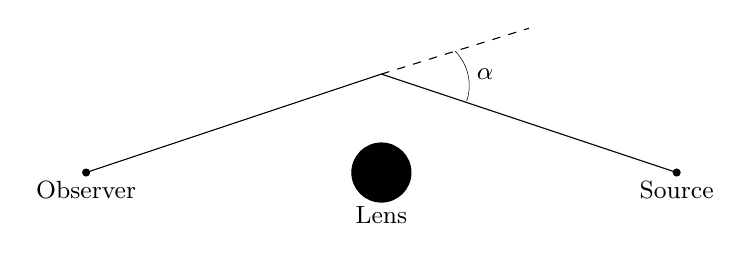
\begin{tikzpicture}[scale=1.25,>=stealth]
    \small
    \filldraw (0,0) circle (3mm)
      node[below=9] {Lens};
    \filldraw (-3cm,0) circle (1pt)
      node[below] {Observer};
    \filldraw (3cm,0) circle (1pt)
      node[below] {Source};
    \draw[thin] (-3cm,0) -- (0,1cm);
    \draw[thin,dashed] (0,1cm) -- (1.5cm,1.466cm);
    \draw[thin] (0,1cm) -- (3cm,0);
    \draw[very thin,yshift=1cm] (7.5mm,2.33mm) arc (44.34:-18.43:5mm)
      node[midway,right] {$\alpha$};
  \end{tikzpicture}
\end{figure}

\begin{figure}
  \caption{\label{fig:imgbuild}
    Illustration marking intermediary steps during the image forming process.
    First, a new image is generated as a default, black canvas of the same resolution as the input image.
    Then, during execution the algorithm used by our \python{apply\_lensing} method iterates through each pixel of the newly generated image and uses the passed lensing map to determine which pixel from the input should be placed at that location.
}
  \vspace{3mm}
  \begin{tikzpicture}[>=stealth,line width=3pt]
    \tikzset{every node/.style={inner sep=0pt}}
    \def\voffset{3.75cm}
    \def\hoffset{5cm}
    \node (in) at (-\hoffset,0pt)
      {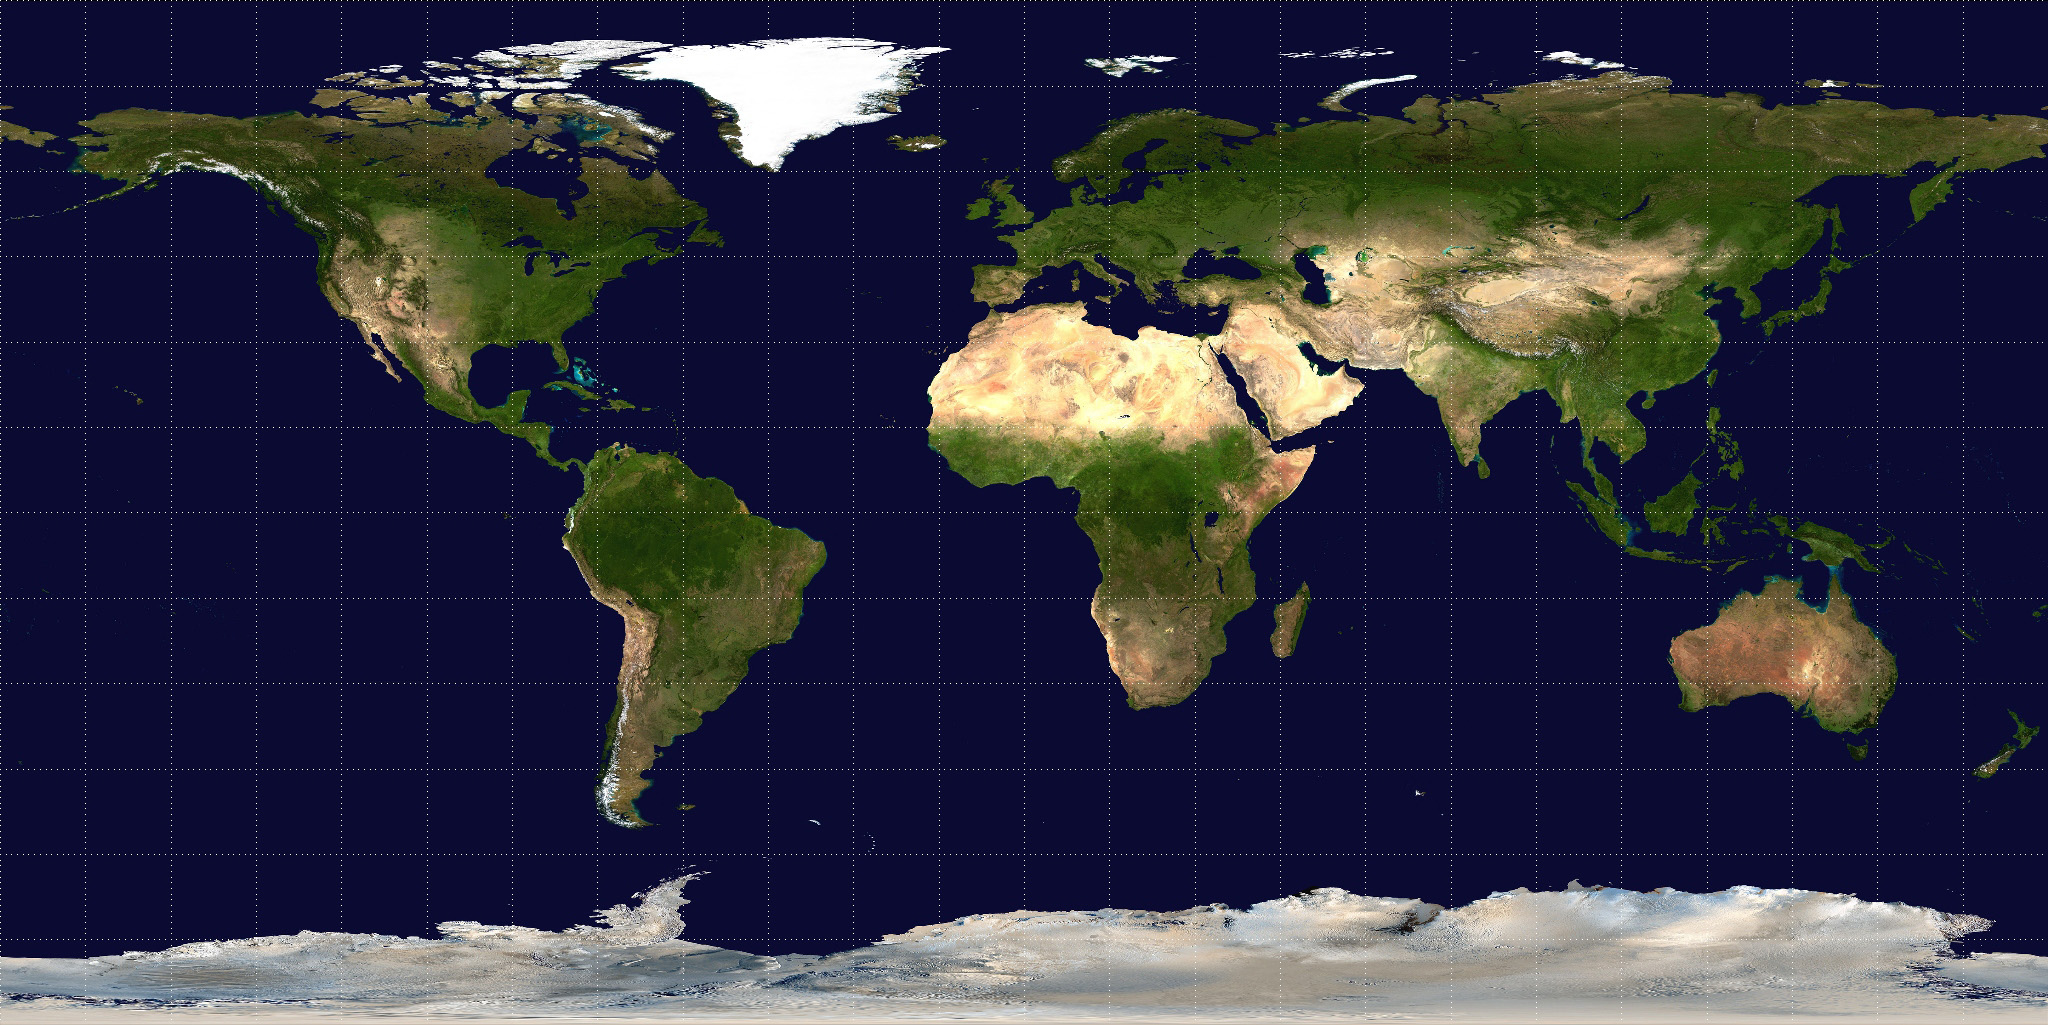
\includegraphics[width=.4\textwidth]{earth}};
    \node (out1) at (\hoffset,\voffset)
      {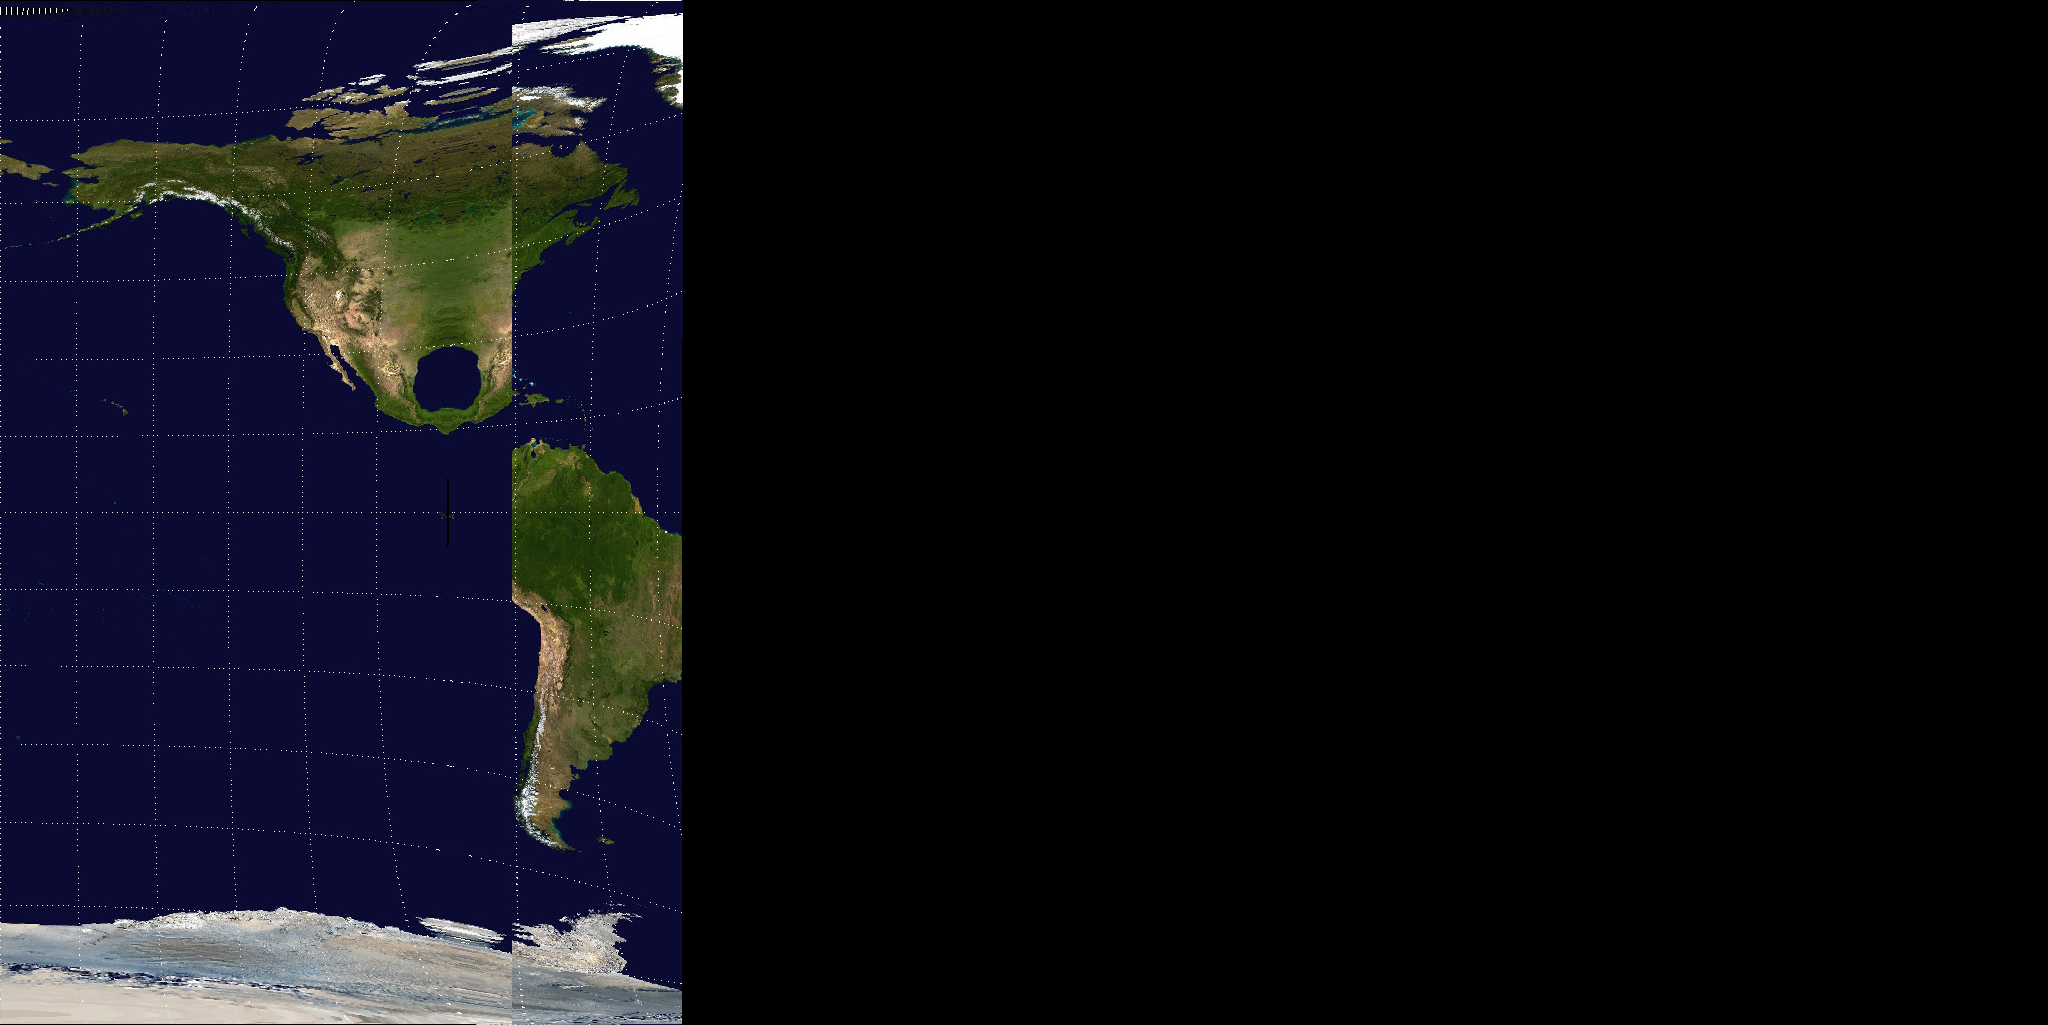
\includegraphics[width=.35\textwidth]{output_onethird}};
    \node (out2) at (\hoffset,0pt)
      {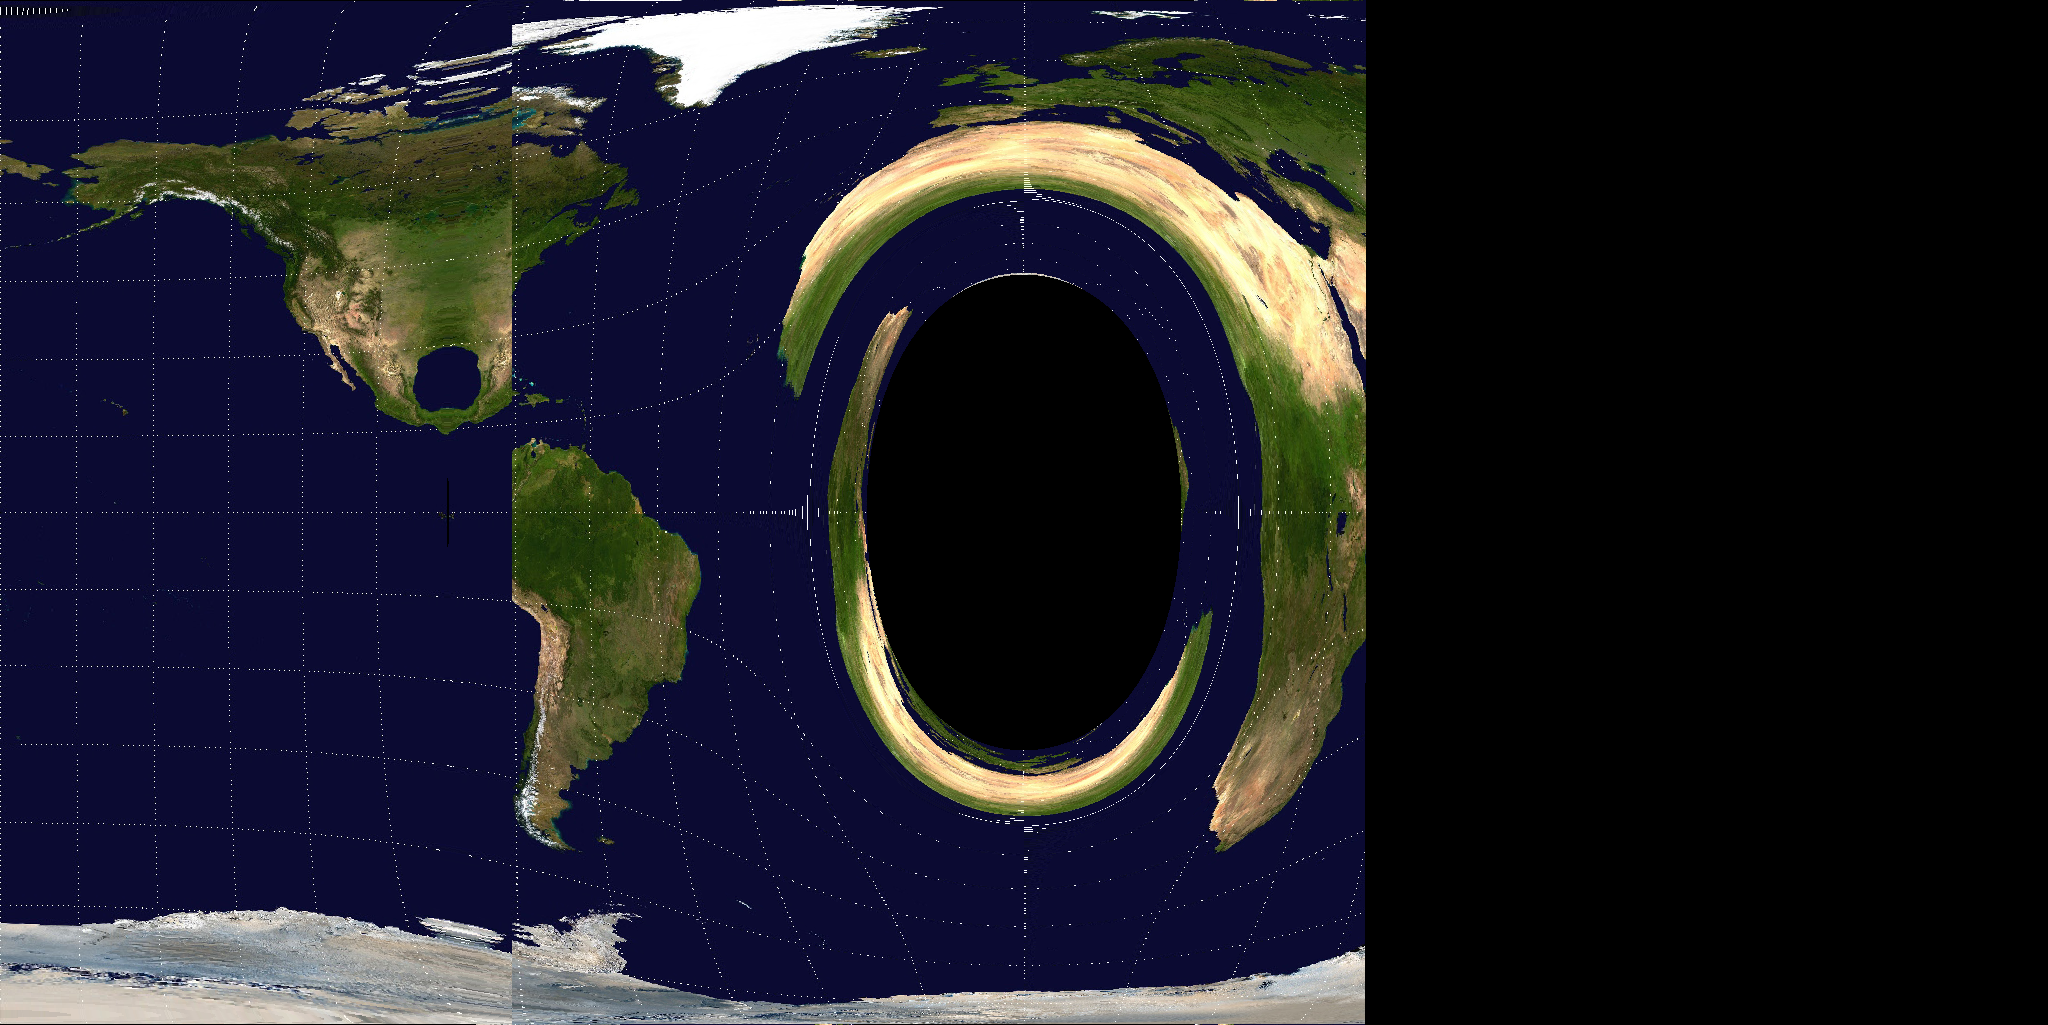
\includegraphics[width=.35\textwidth]{output_twothird}};
    \node (out3) at (\hoffset,-\voffset)
      {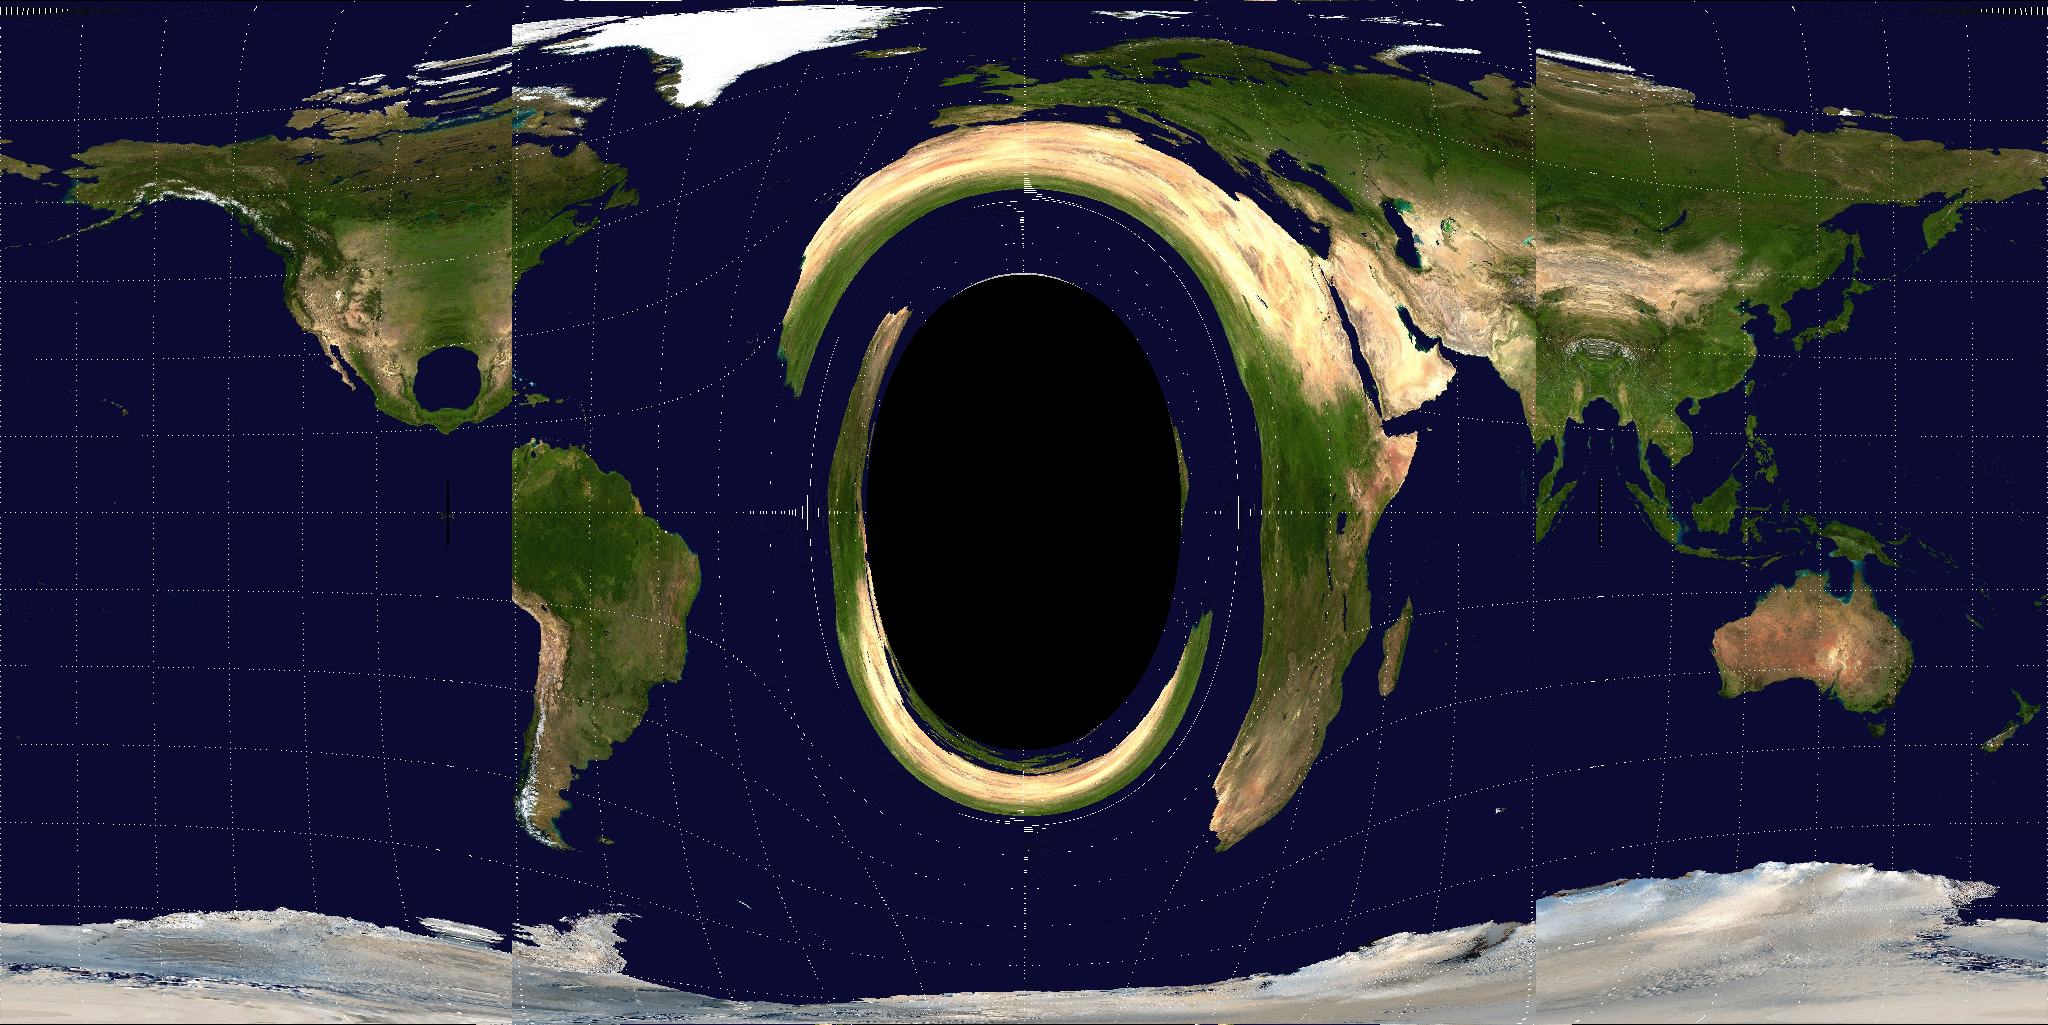
\includegraphics[width=.35\textwidth]{output_full}};
    \draw[->,shorten <=5mm,shorten >=5mm] (in) -- (out2);
    \draw[->] (out1) -- (out2);
    \draw[->] (out2) -- (out3);
  \end{tikzpicture}
\end{figure}

\end{document}
